% =====================================================================
%  AAAI-27 DEMONSTRATION TRACK SUBMISSION
%
%  Format per the AAAI-27 Call for Demonstrations:
%    - two-page short paper describing the system
%    - plus ONE page of references only
%    - AAAI two-column style (AuthorKit27)
%    - accompanied by a video of up to 5 minutes (submitted separately
%      as supplementary material in OpenReview)
%
%  Reviewing is single-blind OR double-blind, author's choice.
%  This file is set up SINGLE-BLIND (author names visible), which lets
%  the production-deployment context do its work.
%  To switch to double-blind: change \usepackage{aaai2027} below to
%  \usepackage[submission]{aaai2027} and the names are suppressed.
%
%  Terminology: three "gates" (the longer RE-XTRACT manuscript calls them
%  "layers" -- align it if both papers go out); N concurrent SAMPLES of one
%  model, never "agents".
%
%  Build:  latexmk -pdf main.tex
% =====================================================================

\documentclass[letterpaper]{article} % DO NOT CHANGE THIS
\usepackage{aaai2027}  % DO NOT CHANGE THIS
\usepackage[hyphens]{url}  % DO NOT CHANGE THIS
\usepackage{graphicx} % DO NOT CHANGE THIS
\urlstyle{rm} % DO NOT CHANGE THIS
\def\UrlFont{\rm}  % DO NOT CHANGE THIS
\usepackage{natbib}  % DO NOT CHANGE THIS AND DO NOT ADD ANY OPTIONS TO IT
\usepackage{caption} % DO NOT CHANGE THIS AND DO NOT ADD ANY OPTIONS TO IT
\frenchspacing  % DO NOT CHANGE THIS

\usepackage{booktabs}
\usepackage{amssymb}
\usepackage{tikz}
\usetikzlibrary{arrows.meta,positioning,calc}

% --- Figure 1 palette (xcolor is already loaded by aaai2027.sty) ------
\definecolor{rxteal}{RGB}{31,110,120}
\definecolor{rxtealmid}{RGB}{60,148,156}
\definecolor{rxtealbg}{RGB}{226,243,243}
\definecolor{rxsalm}{RGB}{221,116,88}
\definecolor{rxsalmbg}{RGB}{253,233,225}
\definecolor{rxnavy}{RGB}{68,86,146}
\definecolor{rxnavybg}{RGB}{227,231,245}

\pdfinfo{
/TemplateVersion (2027.1)
}

\setcounter{secnumdepth}{0}

% System name --- change here and it changes everywhere.
\newcommand{\sys}{RE-XTRACT}

\title{\sys: Unanimity-Gated Document Extraction with Calibrated Abstention}

\author{
    Harshul Kuhar,
    Harshit Oberoi
}
\affiliations{
    Housing.com\\
    Gurugram, India\\
    \{harshul.kuhar@housing.com, harshit.oberoi@housing.com\}
}

\begin{document}
\maketitle

\begin{abstract}
In information extraction from unstructured documents, errors have asymmetric costs: a wrong
value silently corrupts downstream databases. Although vision-language models
(VLMs) are capable of reading document contents with high proficiency, they cannot
reliably flag their own mistakes. We introduce \sys, an extraction
system designed for Indian real-estate regulatory (RERA) filings. 
To prevent silent failures, \sys{} classifies documents and extracts
a fixed schema of dates and building-scope fields using three composable gates 
over an open-weight VLM:
(1) exact-match consistency across $N$ voting rounds, (2) independent validation
of unanimous consensus by a frontier model, and (3) a final fallback that
safely abstains when they disagree. On a 143-document production benchmark,
\sys{} classifies documents with 95.1\% accuracy  against
85.3\% for a previous generator-verifier pipeline, and reads 95.6\% of
113 gold dates correctly against 88.5\%. 
We demonstrate \sys{} live, letting users process
documents and inspect decision provenance in
real time.


\end{abstract}

\begin{links}
  \link{Demo}{https://taxonomic-unadversely-zonia.ngrok-free.dev}
\end{links}

% =====================================================================
\section{Introduction}

\begin{figure}[t]
\centering
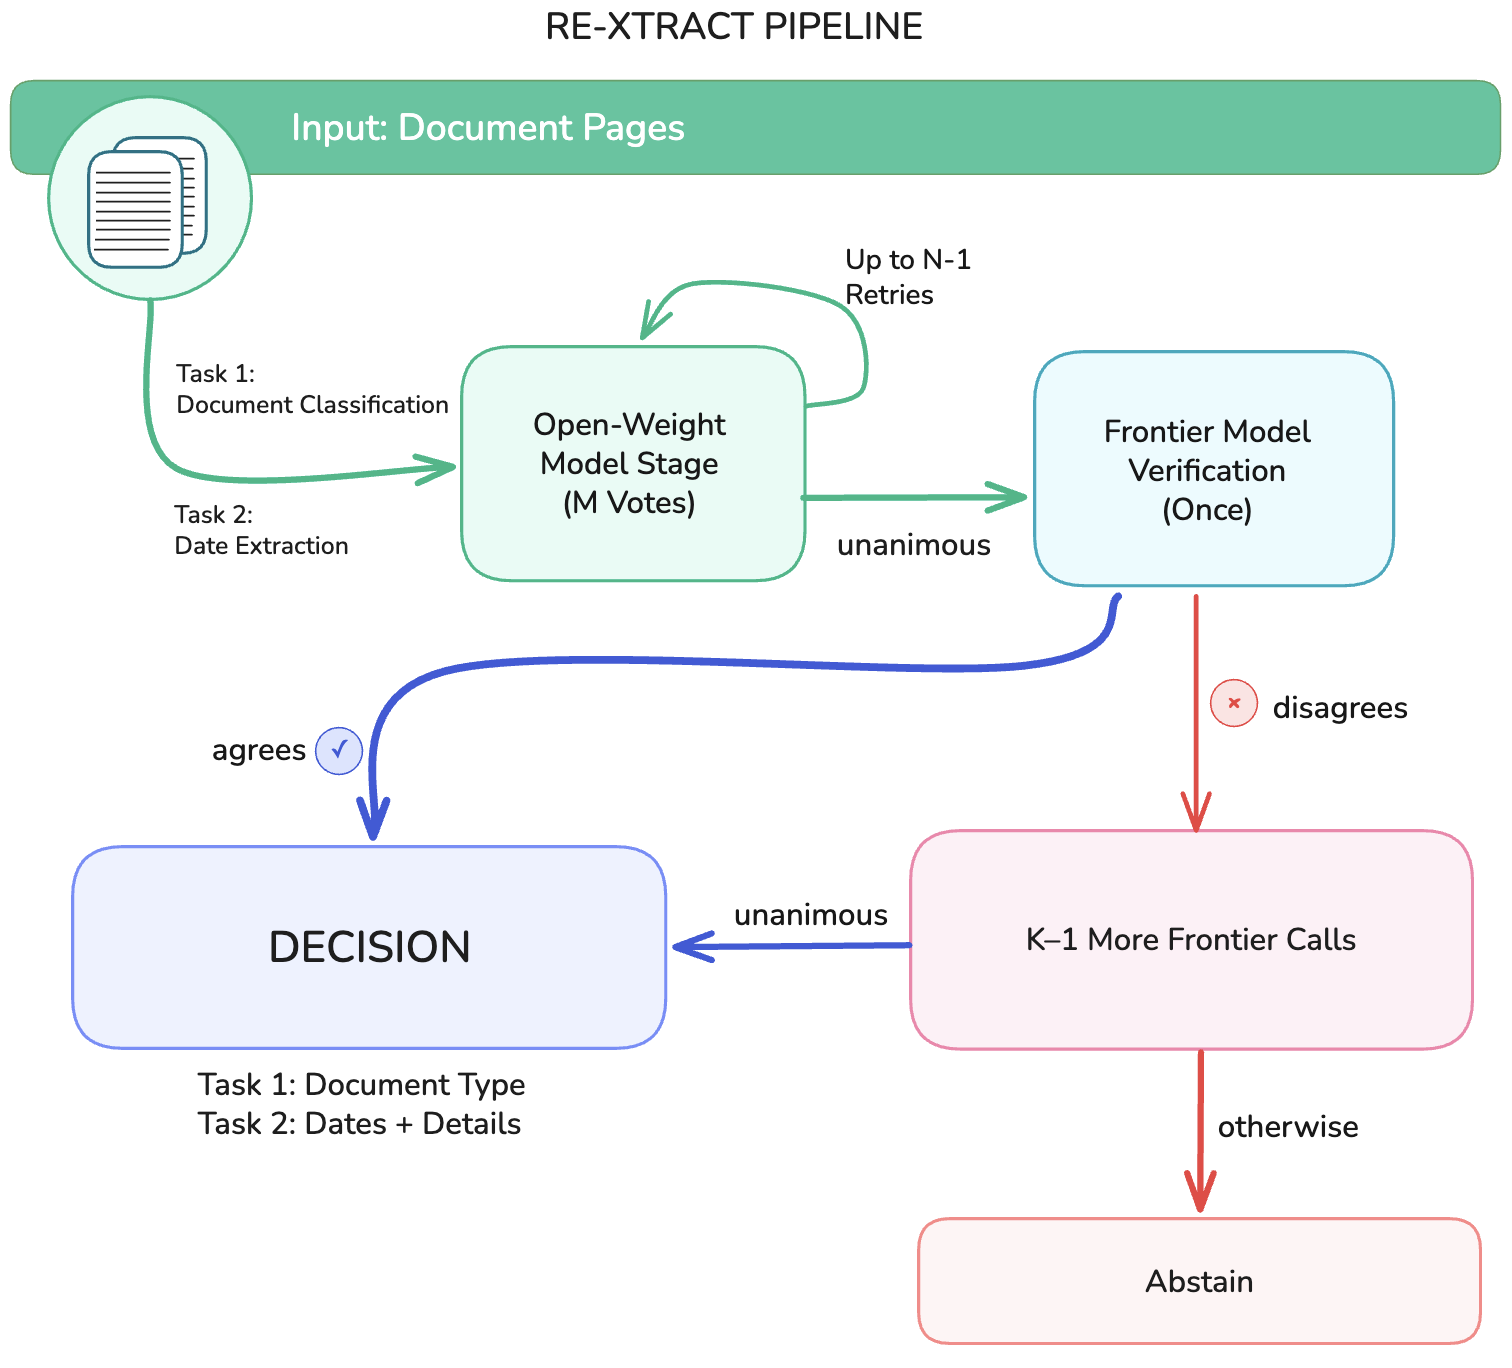
\includegraphics[width=0.95\columnwidth]{data/rextract_flow.png}
\caption{The \sys{} pipeline. A round of $M$ votes from one open-weight
model must be unanimous, with up to $N{-}1$ retries, before a frontier
model checks the answer. A rejected answer escalates to $K$ frontier calls
in total, and anything still unresolved abstains.}
\label{fig:arch}
\end{figure}

Whether a real-estate project in India is on schedule, delayed or
delivered is largely invisible to the homebuyers and investors who
depend on it. The Real Estate (Regulation and Development) Act, 2016
(RERA) addresses this trust gap by requiring
every real-estate project in India to register with its state regulatory
authority and to keep a public document trail. In practice this trail is
a directory of scanned PDFs per project, uploaded by promoters and
authorities over the project's lifetime. Four document types carry the
information that downstream products actually need:
\begin{itemize}
  \item \textbf{Registration Certificate (RC)} - establishes the
        project and states the date on which registration was granted
        and the date by which the promoter has promised completion.
  \item \textbf{Extension Certificate (EC)} - issued later, moves the
        promised completion date in cases of delay.
  \item \textbf{Occupancy Certificate (OC)} - a municipal body
        certifies a building is fit for occupation.
  \item \textbf{Completion Certificate (CC)} - a municipal body
        certifies construction is complete and conforms to plan.
\end{itemize}

Altogether, these dates are the ground truth for a listed project's current and
future status; extracting them, however, is not trivial. A single project's filings 
run to hundreds of documents, most of which - GST registrations, Water certificates, 
handover deeds - carry none of these dates. Moreover, the relevant certificates follow 
no common format, and some are handwritten.

Several works explore Optical Character Recognition (OCR) technique for extraction of fields
from documents~\citep{zhang2024docparsing}, but the nature of unstructured documents renders them unsuitable. Instead,
vision-language models (VLMs) have gained traction, since they read a page directly as an
image and thus absorb layout variation that a fixed OCR pipeline cannot~\citep{han2025mdocagent}.
Additionally, established OCR toolkits are themselves converging on this design: PaddleOCR-VL
folds a 0.9B-parameter VLM into the parsing stack in place of a staged recogniser, which enables 
it to parse across 109 languages~\citep{cui2025paddleocrvl}.

A single VLM call, however, yields no signal that separates a correct reading from an
incorrect one. A date transcribed from the wrong document is as fluent as the true value.
The two errors are not equally costly in this setting; an omitted date can be
re-queued, but an erroneous one is republished as the project's official status.

This asymmetry shapes \sys. The system follows the principle of \emph{Agreement-as-a-Confidence} 
by sampling one model repeatedly and requiring exact
agreement before corroborating it across a second model, and abstaining when
neither holds. Sampling consistency is a known
fabrication signal~\citep{wang2023selfconsistency,manakul2023selfcheckgpt};
\sys{} composes it with cross-model corroboration with an explicit reject
option~\citep{geifman2017selective,kamath2020selective}, and preserves the entire decision 
history for auditable tracking.

% =====================================================================
\section{System Overview}

\sys{} takes a RERA ID and collects the project's filed documents.
Figure~\ref{fig:arch} shows the pipeline, a fixed LangGraph state machine.
Each document is ran in two stages - it is first classified into one of the four
certificate types, and then routed to its own schema of dates and details.
Both decisions pass through the same three gates below.

\paragraph{1. Ingest:}
Documents are rendered to page images at 150\,DPI and deduplicated using
MD5 for byte-identical PDFs, and perceptual hash for visually
identical rescans.

\paragraph{2. Voting:}
The pages are put to a self-hosted open-weight VLM $M$ times, giving $M$ votes
on the decision at hand. On the extraction pass, dates are copied verbatim and
converted to ISO form (YYYY-MM-DD) by a deterministic parser, so votes are
compared on value rather than wording. The votes are then checked for a
unanimous match; if they disagree, the round is retried up to $N{-}1$ times,
lasting at most $N$ rounds.

\paragraph{3. Verification:}
Unanimity among votes from one model is not enough on its own, since a
small model can be consistently wrong. When a round is unanimous, \sys{}
puts the same question to a frontier model over the same pages. If its answer
matches the unanimous one, the answer is final.

\paragraph{4. Escalation and Abstention:}
If the frontier model disagrees, \sys{} calls it $K{-}1$ more times and
checks all $K$ answers for unanimity. If they agree, that answer is
final. Otherwise \sys{} abstains: a classification decision sets the document aside,
an extraction decision writes no value, and either is terminal. $K$ is capped
separately from $M$ because frontier calls are metered and local votes are
not.

If any of the gates abstain from answering, the document is skipped, or flagged
for manual review.

% =====================================================================
\section{Demonstration}

Our demo shows the full extraction workflow on a fixed corpus of RERA
filings. A visitor selects one of six preloaded projects and the pipeline
runs on it in-real time. The interface shows each of the $M$ votes as the open-weight 
model is called accompanied by the frontier model's verdict, and subsequent flows upon disagreement.
The complete process is shown in the demo video.

% =====================================================================
\section{Deployment and Results}

\sys{} runs in production at Housing.com, writing RERA filings into a Delta
Lake table behind consumer-facing project timelines. The local
model is a 2.3B-parameter model from the Qwen 3.5
family~\citep{bai2023qwenvl}; the frontier model is
gemini-2.5-flash-lite~\citep{comanici2025gemini25}. We evaluate classification on 143
documents from production traffic, covering 47 projects across seven
states.

Table~\ref{tab:results} compares \sys{} against the generator-verifier
loop~\citep{madaan2023selfrefine}, in which one call
extracted and a second call verified until the two agreed. Classification accuracy rises
from 85.3\% to 95.1\% and Macro-F1 score from .804 to .955. Biggest improvement is in classification 
of out-of-schema documents, where the recall moves from .32 to .93, so the documents
that should have been turned away are now correctly flagged. Precision on
this class, however, drops from 1.00 to .84, which is an acceptable tradeoff, since this is an 
error that costs an operator a second look rather than a corrupted record.


The lower panel of Table~\ref{tab:results} reports the date extraction stage. Over 113 gold dates from the
same projects, \sys{} reads 108 correctly against 100 for the
generator-verifier loop, raising date accuracy from 88.5\% to 95.6\%.


\begin{table}[t]
\centering
{\small
\begin{tabular}{lcccccc}
\toprule
& \multicolumn{3}{c}{Gen.-verifier} & \multicolumn{3}{c}{\sys} \\
\cmidrule(lr){2-4} \cmidrule(lr){5-7}
Class & P & R & F1 & P & R & F1 \\
\midrule
\multicolumn{7}{l}{\emph{Stage 1: Document Classification}} \\
Registration     & .98 & .96  & .97 & \textbf{1.00} & \textbf{.98} & \textbf{.99} \\
Extension        & .80 & 1.00 & .89 & \textbf{1.00} & 1.00 & \textbf{1.00} \\
OC / Completion  & .78 & 1.00 & .87 & \textbf{.97} & .94 & \textbf{.95} \\
Out-of-schema    & 1.00 & .32 & .49 & .84 & \textbf{.93} & \textbf{.88} \\
\midrule
Accuracy & \multicolumn{3}{c}{85.3\%} & \multicolumn{3}{c}{\textbf{95.1\%}} \\
Macro-F1 & \multicolumn{3}{c}{.804} & \multicolumn{3}{c}{\textbf{.955}} \\
\midrule
\multicolumn{7}{l}{\emph{Stage 2: Date Extraction, 113 gold dates}} \\
Correct       & \multicolumn{3}{c}{100}    & \multicolumn{3}{c}{\textbf{108}} \\
Incorrect     & \multicolumn{3}{c}{13}     & \multicolumn{3}{c}{\textbf{5}} \\
Accuracy      & \multicolumn{3}{c}{88.5\%} & \multicolumn{3}{c}{\textbf{95.6\%}} \\
\bottomrule
\end{tabular}}
\caption{Both gated stages, compared against the earlier generator-verifier
pipeline. Classification covers the 143-document benchmark (45 Registration, 8
Extension, 62 Occupancy/Completion, 28 out-of-schema); date extraction covers
113 gold dates from the same projects.}
\label{tab:results}
\end{table}



% =====================================================================
\section{Conclusion}

We present \sys{}, that treats agreement as its only evidence of correctness: a local
model must vote unanimously, a frontier model must confirm it, and anything
unresolved is set aside, not guessed. In production, that is 95.1\%
classification accuracy and 95.6\% on dates.

% =====================================================================
% NOTE: aaai2027.sty already sets the bibliographystyle. Adding an explicit
% \bibliographystyle command here is an error (AuthorKit27 instructions).
\bibliography{refs}

\end{document}
